\documentclass{beamer}
\beamertemplatenavigationsymbolsempty
\usepackage{amsmath, amssymb, hyperref, graphics, tikz}
\usepackage[normalem]{ulem} %for strikeout \sout{ }

\usepackage{tikzsymbols} %for smileys

\newcommand{\C}{\mathbb{C}}
\newcommand{\Z}{\mathbb{Z}}
\newcommand{\R}{\mathbb{R}}
\newcommand{\N}{\mathbb{N}}
\DeclareMathOperator{\Real}{Re}
\DeclareMathOperator{\Imag}{Im}
\DeclareMathOperator{\Res}{Res}
\begin{document}


\begin{frame}{Announcements}

  \begin{block}{\Xey Strike \Xey}
\begin{itemize}
  \item (First wave?) Next Week, December 1,2,3
  \item GLobal Issues: Pensions, Four Fights
  \item Local Issues: Archaeology, Modern Languages  
\end{itemize}
  \end{block}

  \begin{block}{Other items}
\begin{itemize}
  \item Can still hand in second homework for feedback
  \item Exam still being finalized, more information soon
    \item  Finish notes next week!  Revision topics?
    \item Will have office hours + revision sessions in January
\end{itemize}
\end{block}

  \begin{block}{Home stretch:}
Preparing for the Residue Theorem
      \end{block}
\end{frame}  

\begin{frame}{Laurent Series: First example}
  For $|z|<1$, we have
  $$\frac{1}{1-z}=1+z+z^2+z^3+\cdots$$
  As $|z|\to\infty, \frac{1}{1-z}\to 0$.  Can we analyze how?

  \begin{block}{Yes!}
    As $|z|\to\infty, |1/z|\to 0$, and in particular $|1/z|<1\dots$
  \end{block}

\end{frame}

\begin{frame}{Laurent Series: Definition}
  A Laurent series about $a$ is a like a Taylor Series but where we also allow negative powers.
  \begin{definition}

  A Laurent series around $a$ is a series of the form
  $$\sum_{n=-\infty}^\infty a_n(z-a)^n$$
If the series converges to a function $f(z)$ for $0<|z-a|<r$, the coefficient $a_{-1}$ is called the \emph{residue of $f$ at $a$}.
  \end{definition}
  
  Generally will converge on some (perhaps empty) annulus $r<|z-a|<R$, and give a holomorphic function there.
 
\begin{block}{Why?}  
  \begin{itemize}
  \item Replacement for Taylor series around isolated singularities
    \item Easy to integrate over a contour around $a$
\end{itemize}
 \end{block}
 \end{frame} 



\begin{frame}{Classification of Singularities}
By Laurent's Theorem, if $f(z)$ is analytic in a punctured disk around $\alpha$, it has a convergent Laurent expansion
$$f(z)=\sum_{n\in\Z} a_n (z-\alpha)^n$$
\begin{block}{Three possibilities:}
\begin{description}
   \item[Removable singularity] None of the $a_n$ with $n<0$ are nonzero
       \item[A pole] Only finitely many $a_n$ with $n<0$ are nonzero
    \item[Essential singularity] Infinitely many $a_n$ with $n<0$ are nonzero

\end{description}
\end{block}

\begin{block}{Punchline first:}
Only for essential singularities will you need to compute the Laurent series to find the pole!
\end{block}

\end{frame}


\begin{frame}{Removable singularities: no negative powers}
$f$ has a removable singularity at $\alpha$ means it has no negative powers of $z-\alpha$ in its Laurent series.  

But then it's Laurent series is really a Taylor series, and it makes sense to plug in $\alpha$.  Thus $f$ extends to an analytic function around $\alpha$.  
\begin{block}{Examples:}
\begin{enumerate}
\item $\frac{z^2-1}{z-1}$
\item $\frac{\sin(z)}{z}$
\end{enumerate}
\end{block}

Since the Laurent series has no negative powers, the residue of a removable singularity is always zero.
\end{frame}


\begin{frame}{Poles: only finitely many negative terms}
\begin{definition}
We say that $f(z)$ has a \emph{pole of order $k$} at $\alpha$ if its Laurent series $f(z)=\sum_{n\in\Z} a_n(z-\alpha)^n$ has $a_{-k}\neq 0$, but $a_{n}=0$ for $n<-k$.
\\ ~ \\
In other words
$$f(z)=\sum_{n\geq -k} a_n (z-\alpha)^n$$
A pole of order one is also called a \emph{simple pole}.
\end{definition}
\begin{block}{Examples: poles of order 2} 
\begin{enumerate}
    \item $\frac{e^z}{z^2}$
    \item $\tan^2(z)$
  \end{enumerate}
\end{block}


\end{frame}


\begin{frame}[plain]
\begin{columns}
\begin{column}{0.5\textwidth}
    
\includegraphics[width=\textwidth,height=\textheight,keepaspectratio]{PolePun.jpg}
\end{column}
\begin{column}{0.5\textwidth}
\begin{block}{Poles of the gamma function}
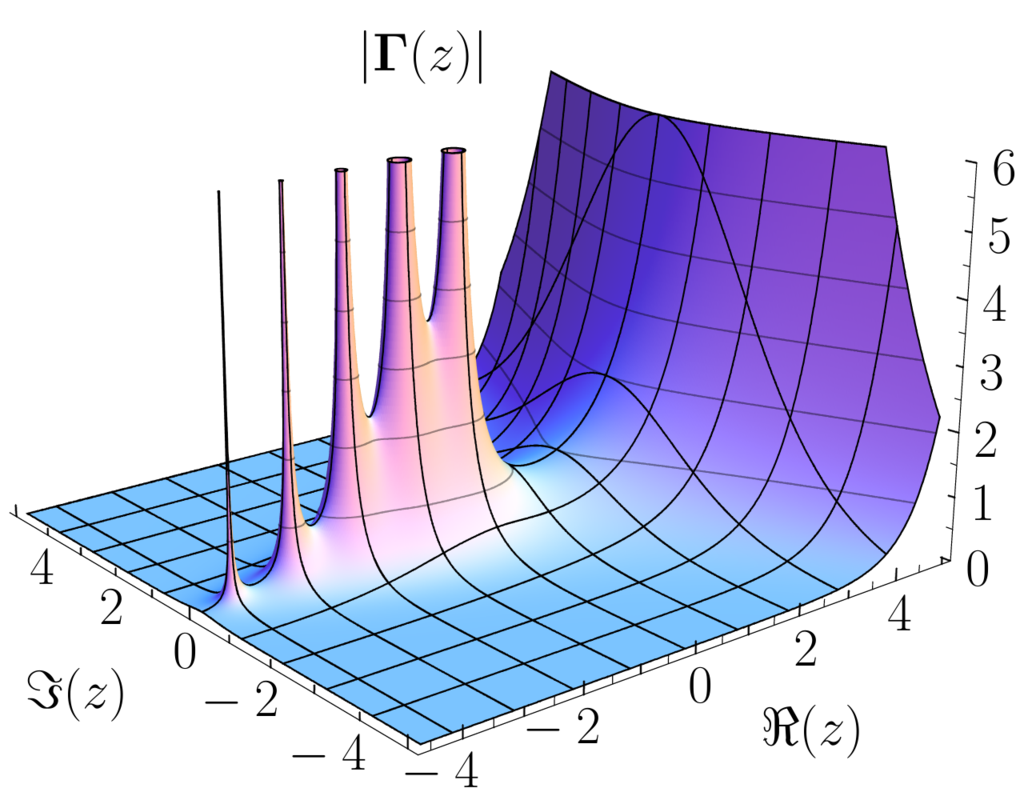
\includegraphics[width=\textwidth,keepaspectratio]{GammaPoles.png}
$\Gamma(z)$ extends $(n-1)!$ to an analytic function, and has simple poles at the non-positive integers
\end{block}
\end{column}
\end{columns}

\end{frame}
\begin{frame}{Essential singularity: infinitely many negative powers}
\begin{definition} If the Laurent series of $f(z)$ around $\alpha$ has infinitely many $a_{k}\neq 0$ with $k<0$, then we say $\alpha$ is an \emph{essential singularity} of $f$\end{definition}


\begin{examples}
\begin{itemize}
    \item $e^{1/z}$
    \item $\cosh(1/z)$
\end{itemize}
\end{examples}

\begin{theorem}[Great Picard's Theorem -- just for culture]
If $f(z)$ has an essential singularity at $\alpha$, then on any punctured disk around $\alpha$, $f(z)$ takes on all possible complex values, with at most one exception, infinitely often.
\end{theorem}
So $\lim_{z\to\alpha} |f(z)|=\infty$ for a pole, but horribly doesn't exist for an essential singularity.

\end{frame}

\end{document}


\begin{frame}{Easy (and examinable!) theorems about poles}
\begin{theorem} $f$ has a pole of order $k$ at $\alpha$ if and only if $$f(z)=\frac{g(z)}{(z-\alpha)^k}$$ where $g(z)$ analytic and nonzero in some disk around $\alpha$.
\end{theorem}

\begin{theorem} If $f$ has a zero of order $k$ at $\alpha$, then $1/f$ has a pole of order $k$ at $\alpha$.
\end{theorem}

\begin{corollary}If $f$ has a zero of order $m$ at $\alpha$, and $g$ has a zero of order $n$ at $\alpha$, then
\begin{itemize}
    \item $\frac{f}{g}$ has a pole of order $n-m$ if $n>m$
    \item $\frac{f}{g}$ has a removable singularity if $m\geq n$
\end{itemize}
\end{corollary}
\end{frame}

\begin{frame}{Easy way to find residues at poles}
\begin{theorem}
Suppose that $f$ has a pole of order $k$ at $\alpha$.  Then

$$\Res\{f;\alpha\}=\frac{1}{(k-1)!}\lim_{z\to\alpha} \frac{d^{k-1}}{dz^{k-1}} (z-\alpha)^kf(z)$$
\end{theorem}
\begin{proof}Just compute the right hand side.
\end{proof}
\begin{corollary}
If $f=g/h$, where $g$ and $h$ are analytic at $\alpha$, $g(\alpha)\neq 0, h(\alpha)=0, h(\alpha)\neq 0$, then $f$ has a simple pole at $\alpha$ and
$$\Res\{f;\alpha\}=\frac{g(\alpha)}{h^\prime(\alpha)}$$
\end{corollary}
\end{frame}



